% !TEX program = xelatex
% !TEX options = -shell-escape
% !TEX options = -8bit

\documentclass[10pt]{scrartcl}
\usepackage[dvipsnames]{xcolor}
\usepackage{fourier}
\usepackage{geometry}
\usepackage[style=authoryear,backend=biber]{biblatex}
\usepackage{tikz}
\usepackage{minted}
\usepackage{mdframed}
\usepackage{fontspec}
\usepackage{listings}
\usepackage{caption}
\usepackage{hyperref}

\definecolor{backcode}{HTML}{404040}
\setmonofont{Source Code Pro}

\usemintedstyle{vs}

\addbibresource{ref.bib}

\setlength\bibitemsep{1.5\itemsep}

\definecolor{bluegray}{HTML}{456B9D}

\hypersetup {
	colorlinks	= true,
	urlcolor  	= bluegray,
	filecolor		= bluegray,
	linkcolor		= bluegray,
	citecolor		= bluegray
}

\begin{document}
	
	\begin{titlepage}
		
		\begin{centering}
		\large Swinburne University of Technology
		\par
		\large COS20007 - Object-Oriented Programming

		\vspace{4cm}

		\Huge \textbf{Data-Oriented, Entity-Component-Systems Within The Context of Object-Orientated Programming}

		\vspace{3cm}

		\Large JACOB MILLIGAN
		\par
		\Large 100660682
		\par

		\vfill

		\today

		\end{centering}



		\begin{tikzpicture}
			
		\end{tikzpicture}

	\end{titlepage}

	\tableofcontents

	\clearpage

	\section{Overview} % (fold)
	\label{sec:overview}

	Object-Oriented programming languages are amongst the most commonly used for developing large software applications \parencite{stack-survey}. Specifically, within the context of video games, the use of C++ as the language of choice is ubiquitous. Game engines commonly have a high demand on resources, frequently operate an a huge variety of data, and encapsulate a large spectrum of disciplines, and often an Object-Oriented approach to design is the most obvious choice for managing complexity. However, as these applications and tools become larger and the demand they place on computer hardware increases, the focus on traditional Object-Oriented design has recently fallen under criticism, not only within the game industry but other software engineering disciplines, as a source of both inefficient run-times and difficult to understand code-bases \parencite{llopis}. 

	In response to these criticisms, many developers within the game industry have turned to a different approach to software architecture - Entity-Component-Systems (ECS) and a 'Data-Oriented' approach to design, both of which aim to decouple program logic from the data it operates on, increase runtime efficiency by maximizing smart CPU caching behavior, and build more flexible, easier to maintain solutions for primarily video-game related, large-scale systems.
	
	This report will explain how Object-Oriented programming is traditionally used within game engines, describe an implementation of an alternate Data-Oriented and Entity-Component based system, and analyze whether the use of such systems and design practices provide a more desirable solution than traditional Object-Oriented design or if a combination of the two approaches is most ideal in relation to run-time efficiency, flexibility, and maintainability.

	\section{Background} % (fold)
	\label{sec:background}
	

	\subsection{Object-Oriented Programming in Games} % (fold)
	\label{sec:object_oriented_programming_in_games}
	Within the game industry C++ is the programming language of choice \parencite[4]{gregory-cpp-usage} and its Object-Oriented features are often heavily utilized for reducing code complexity and encapsulating data. Game objects may have hundreds of variations of their base representation, leading to developers employing inheritance and polymorphic designs that accurately describe the way the game world appears to the user. For example, within the context of Unreal Engine 4, all objects that can be placed within a level inherit from a child of the \mintinline{cpp}{AActor} class which itself is derived from the \mintinline{cpp}{UObject} class \parencite{unreal-docs}, allowing the programmer derive from these classes for their own types and obtain access to a large number of pre-defined behaviors. From the perspective of a user, this can often be the simplest way to express a game engine, however such an approach to design can lead to overly complex code bases as variations in game object types become wide and numerous, resulting in structures similar to Figure ~\ref{fig:ue4}. 
	If not managed carefully by both developers building and using the engine, such structures can become difficult to debug and reason about, performance bottle-necks hard to identify, and modifications to the structure can be challenging as these large hierarchies with many co-dependencies often prove inflexible. 

	\begin{figure}[H]
		\centering
		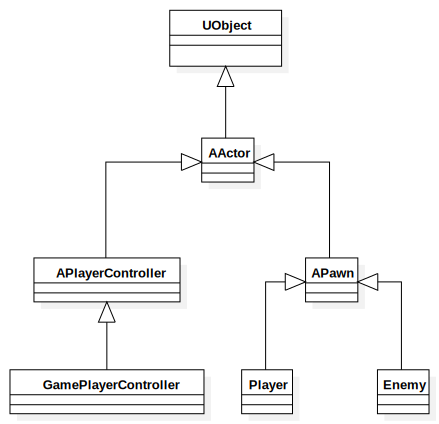
\includegraphics[width=0.7\textwidth]{models/ClassDiagram1.png}
		\caption{A possible Unreal Engine 4 class hierarchy.}
		\label{fig:ue4}
	\end{figure}

	It's important to note that while overly complex and coupled OOP architecture can result in the above-mentioned challenges, relationships between the level of usage of OOP and programmer productivity have been identified \parencite{oop-productivity} \parencite{comstock}, demonstrating that an appropriately decoupled and well-designed Object-Oriented architecture tends to lead to quicker development times. Moreover, this isn't to say that existing engines are poorly designed, only that creating a well-structured solution within them may often be challenging.

	% subsection object_oriented_programming_in_games (end)

	\subsection{Data-Oriented Design} % (fold)
	\label{sub:data_oriented_design}

	\paragraph{CPU Caches} % (fold)
	\label{par:cpu_caches}
	Typically, a CPU will employ a hierarchy of caches of differing speeds and sizes which store recently accessed data for further use in fixed-size blocks known as \textit{cache lines}. Before retrieving some set of data from main memory, the CPU checks for its existence in ascending order in the L1 cache, the smallest and fastest cache, through to the L2 cache and so on before proceeding to fetch it from main memory. Furthermore, a CPU's L1 cache is typically split into a dCache (data) and an iCache (instructions), which allows commonly reused \textit{instructions} to be fetched faster. 
	The speed of each cache is highly dependent on its size and as such, the amount of memory each cache level can store is carefully balanced between specific CPU architectures - for example the highest selling current CPU chip according to both Amazon \parencite{amazon} and Newegg Business \parencite{newegg}, Intel's i7-6700K, has a 256kb L1 cache, split 128kb/128kb between data and instructions, a 1024kb L2 cache, and an 8mb L3 cache. Furthermore, the way in which CPU's \textit{predict} how data will be accessed and how they replace the currently cached data based on this prediction can affect performance. These \textit{replacement policies} can involve replacing oldest data first, or newest data first in the case where a memory access pattern resembles an ABCDABCD sequence, or a combination of both of the two alongside other policies \parencite{Al-Zoubi:2004:PEC:986537.986601}.
	% paragraph cpu_caches (end)

	\paragraph{Data-Oriented Design} % (fold)
	\label{par:data_oriented_design}
	Often referred to as a programming paradigm, Data-Oriented Design can rather be defined as a thought process to apply when designing data structures and algorithms. Primarily this design approach involves reasoning about \textit{how data is used by a computer at the hardware level}, by arranging structures and systems so that their associated data is laid out and operated on in a way that the specific behaviors of different computer architectures are fully taken advantage of and penalties caused by factors such as branch-predictions, cache and TLB (Translation Lookaside Buffer) misses, virtual function and container lookups are minimized or eliminated completely. While appearing at first to be a case of premature optimization, games and their engines operate on frametime-limited deadlines and a Data-Oriented approach to design can lead to significant performance gains \parencite{dice-cull}. Often this approach to software design places a large emphasis on operating on data in bulk, stating that it's relatively rare that any piece of data exists as a unique permutation operated on in complete isolation \parencite{dice-intro}.
	This is often implemented by storing data in contiguous containers, such as arrays or packed plain-data structs, where program systems often consist of a single \mintinline{cpp}{for} loop with minimal branching. As game systems very rarely operate on objects individually, this approach can result in repeatedly accessed data to be present in a single CPU cache line for extended periods of time.
	% paragraph data_oriented_design (end)

	% subsection data_oriented_design (end)	
	
	\subsection{Entity-Component Architecture} % (fold)
	\label{sub:entity_component_architecture}

	Entity-Component architectures were initially developed in order to create flat inheritance structures in Object-Oriented languages and to facilitate highly data-\textit{driven} (Not to be confused with Data-Oriented design) game engines and tools - that is, to allow games to be described using tools, data file formats such as JSON and XML, and databases rather than through code \parencite{thief}.
	\par
	In a pure ECS, a game object (entity) is an integer ID which acts as an index into a series of arrays of \textbf{components} which store only plain data and contain no game logic. All logic within such an application is then executed through \textbf{entity systems} which iterate over these component arrays using each entities id as an index for accessing properties to manipulate. Generally the access and modification of entities, systems, and components is controlled via an \textit{entity lookup table or map} which handles creation, destruction and association of entities and components, storing systems and handing them out as needed, \textbf{Figure~\ref{fig:ecsbasic}} shows an overview of this behavior. In practice this allows entities to be modified and their behavior altered with ease as components are attached and detached as needed and provides numerous other benefits as a side-effect of this behavior, such as:
	\begin{enumerate}
		\item Reducing the number of cache misses, and therefore CPU stalls, during game play due to contiguous storage of components and entities.
		\item An entirely flat inheritance structure, creating easily understood and modularized code bases able to be debugged and tested more flexibly.
		\item A game able to be described primarily through data files, databases, and scripting languages able to be modified by non-programmers with ease.
	\end{enumerate}

	\begin{figure}[H]
		\centering
		\includegraphics[width=\textwidth]{models/ecsdiagram.png}
		\caption{A high-level overview of basic ECS functionality.}
		\label{fig:ecsbasic}
	\end{figure}

	% subsection entity_component_architecture (end)

	% section background (end)

	\section{Entity-Component-System Implementation} % (fold)
	\label{sec:entity_component_system_implementation}

	This section describes an implementation for a complete Entity-Component-System but should in no way be considered as the ideal approach. Many game and application developers will have wide and varied requirements and their goals will be very different to the goals specified here, some may require pure performance, while others may place more importance on readability and interface. As such, this ECS can be considered as an overview of possible implementations, a stepping-stone for further exploration into the subject by interested readers.
	
	\subsection{Requirements} % (fold)
	\label{sub:requirements}
	In the design of the ECS, implemented using C++, three factors were of primary concern:

	\paragraph{Run-Time efficiency} % (fold)
	\label{par:run_time_efficiency}

	As mentioned previously, performance of a program is one of the possible major gains from using an ECS. In the implementation outlined in this report, run-time efficiency is considered as \textit{the lowest possible average time to render a frame}.
	
	% paragraph run_time_efficiency (end)

	\paragraph{Flexibility} % (fold)
	\label{par:flexibility}
	
	Another possible advantage of using an ECS is the flexibility that a programs architecture gains - in fact the earliest proponents of Entity-Component style architectures weren't concerned at all with run-time speeds, just the ability for their software to be driven by data description files and tools \parencite{bilas}. In the context of the implementation outlined in this report, flexibility is related to the number of classes, functions, variables, and control flow statements required to alter in order to add and remove entire application systems, essentially - how easy it is to modify a system.
	
	% paragraph flexibility (end)

	\paragraph{Maintainability} % (fold)
	\label{par:maintainability}

	Maintainability is considered an important part of building large-scale software with long life-spans. While games tend to have short lifespans, the engines they use are generally much more mature and are often iterations of much older engines with new names, sometimes having decades worth of technical history and refactoring, such as in the case of id Software's id-Tech \parencite{id-tech}. In order to mitigate the impact of these issues, a core system should aim to maximize maintainability from the point of design. In regards to the ECS implementation high maintainability is considered as isolation of logic and state, the speed at which one can step through call graphs and class trees to discover bugs, and the ease at which a test can be written without needing to expose any internals to the testing suite.
	
	% paragraph maintainability (end)
	% subsection requirements (end)

	\subsection{Implementation} % (fold)
	\label{sub:implementation}

	\paragraph{Components} % (fold)
	\label{par:components}
	In order to guarantee efficient run-times and maximize cache hits, components are stored so that the sequence in which their members are accessed and modified is \textit{contiguous} and kept as such when entities are destroyed, added, and modified. 

	Many implementations will often store components on the entities themselves in a form of hash map for querying an entities contents, resulting in contiguous access to the \textit{entities} but not necessarily to the components. 

	While this is a much simpler solution for querying components, it can negatively impact run-time speeds when executing systems, not only due to non-contiguous storage of components and therefore cache-unfriendly design, but also due to the overhead of a hashing function and the case where entities being removed and inserted leaves fragmentation of memory resulting in lookup time penalties and more cache problems.

	Therefore the solution can be to store a component as an \mintinline{cpp}{std::vector<T>} and query them by indexing into the vector using each components' owning entity id, effectively creating a \textbf{component pool} that allows each component to be reused amongst entities.

	However, this can result in instances where, as components are reassigned, their index no longer matches their associated entities id, demonstrated in \textbf{Figure~\ref{fig:swapnpop_prob}}.

	\begin{figure}[H]
		\centering
		\includegraphics[width=\textwidth]{models/swapnpop.png}
		\caption{The problem of maintaining indexes in an ECS}
		\label{fig:swapnpop_prob}
	\end{figure}

	\par
	In order to resolve this problem, an indirection table can be employed for querying an entity by id, implemented in the \mintinline{cpp}{ComponentData<T> struct}. Essentially this consists of an array of size \mintinline{cpp}{UINT16_MAX} (65535) containing a series of \mintinline{cpp}{Entity struct}s that acts as a level of indirection, much like the index in the back of a book allows you to quickly find \textit{the page} (or index) a particular topic (or piece of data) is located at. This indirection array then returns the index (or page, sticking with the book analogy) that the data (or topic) is located at within the actual \mintinline{cpp}{std::vector<T>} that contains the component instances. As the indirection array always contains the maximum number of possible entities, the id's will always be in their correct position, \textbf{Listing~\ref{lst:lookup}} shows the code for this.

		\begin{listing}[H]
	\begin{minted}[bgcolor=backcode,style=native,breaklines=true]{cpp}
/// ComponentData is a container of components with garunteed contiguous
/// storage that can be queried with an Entity id
/// \tparam Type of component to store
template <typename T>
struct ComponentData {

  /// All instances of this component mapped to an entity
  std::vector<T> instances;

  /// Initializes the container and lookup table with all entities
  ComponentData()
  {
    for ( int e = 0; e < UINT16_MAX; ++e ) {
      lookup_[e].id = e;
      lookup_[e].index = UINT16_MAX;
      lookup_[e].generation = UINT16_MAX;
    }
  }

  /// Gets an entities associated component as a pointer.
  /// Uses a pointer rather than a reference to allow for better
  /// auto compatibility and checking against nullptr
  /// \param entity The entity whose component is being retrieved
  /// \return Pointer to the component instance if found, nullptr otherwise
  inline T* get(const Entity& entity)
  {
    auto lookup = lookup_[entity.id];
    if ( lookup.generation != entity.generation )
      return nullptr;

    return (lookup.index < UINT16_MAX) ? &instances[lookup.index] : nullptr;
  }

private:
  /// Lookup array used to index into the actual data
  Entity lookup_[UINT16_MAX];
};
	\end{minted}
	\caption{Using a lookup array as a level of indirection for maintaining indexes}
	\label{lst:lookup}
	\end{listing}	

	Each element of the indirection array contains an \mintinline{cpp}{Entity struct} where its index is either a valid index in the actual component vector, or if the entity is not present, will have its index set to \mintinline{cpp}{UINT16_MAX}. Whenever an entity is added, a new component is pushed to the back of the component vector and the entity in the indirection array is updated with its new index, when an element is swapped, the two elements involved in the swap are updated in the indirection array with their new indexes and any elements being removed are assigned \mintinline{cpp}{UINT16_MAX} to reflect non-existence, demonstrated in \textbf{Figure~\ref{fig:indirection}}. The code for the implementation can be seen in \textbf{Appendix~\ref{sec:appendix_a_code}}, \textbf{Listing~\ref{lst:component}}.

	\begin{figure}[H]
		\centering
		\makebox[\textwidth][c]{
			\includegraphics[width=1.4\textwidth]{models/indirection.png}
		}
		\caption{Using a layer of indirection to solve the inaccurate id problem}
		\label{fig:indirection}
	\end{figure}

	% paragraph components (end)

	\paragraph{Entities} % (fold)
	\label{par:entities}
	Entities, shown in \textbf{Listing~\ref{lst:entity}}, are designed to be lightweight and passed around the program in much the same fashion that primitive data types are. These are defined as \mintinline{cpp}{struct}s with a single id and index field alongside a \mintinline{cpp}{generation} field which is incremented whenever \mintinline{cpp}{UINT16_MAX} is reached and the \mintinline{cpp}{nextId_} field in the EntityMap (see \textbf{Section~\ref{par:entity_map}}) wraps to 0. This allows for a potential of $2^{256}$ total possible entities over the lifespan of the program while still keeping the entity lightweight - limited in size to 48 bits yet still containing lots of information about their state.
	
	\begin{listing}[H]
	\inputminted[bgcolor=backcode,style=native]{cpp}{code/entity.cpp}
	\caption{Entity definition}
	\label{lst:entity}
	\end{listing}

	% paragraph entities (end)

	\paragraph{Systems} % (fold)
	\label{par:systems}

	Using the above mentioned structures, systems are not required to be formally defined within the ECS and can be as simple as free functions declared in-line. However, part of a good ECS implementation is a good interface to match the usability of traditional OOP designs. Systems are designed to be entirely flexible with the only caveat be that they inherit from the base \mintinline{cpp}{System} class and implement the \mintinline{cpp}{add()}, \mintinline{cpp}{remove()}, and \mintinline{cpp}{has_entity()} abstract member functions to operate on their unique sets of data. These abstract functions are useful as each system may have more than one \mintinline{cpp}{ComponentData} container which may have unique requirements. Moreover, any potential performance hit caused by a single v-table lookup per system retrieval (once per frame) is minimal compared to the hit to programmer productivity that may occur without a defined interface for the whole ECS.

	As a result, systems can be stored in homogeneous containers, allowing entities to have components attached and detached by simply iterating over all systems of interest and calling these polymorphic functions. Furthermore, as each system contains only its data of interest, the length of iteration over entities is limited to the length of its set of components and cache misses can be minimized. A trivial example of one such system is outlined in \textbf{Listing~\ref{lst:movement}}.

\inputminted[bgcolor=backcode,style=native]{cpp}{code/movement.cpp}
\captionof{listing}{An example system which moves all entities \label{lst:movement}}
	
	% paragraph systems (end)

	\paragraph{Entity Map} % (fold)
	\label{par:entity_map}
	As is, systems, components and entities can be operated on in complete isolation without the need for some kind of centralized control or container class as long as careful manual management of entity id's occurs. However, as previously discussed, an approachable and centralized interface is desirable. Therefore, an \mintinline{cpp}{EntityMap} was implemented which maps systems, components, and entities to one another and handles the creation and destruction of entity id's, taking note of current generations and keeping track of the amount of live entities in existence. The EntityMap also stores each system within an \mintinline{cpp}{std::unordered_map<std::type_index, std::unique_ptr<System>>} shown in Listing ~\ref{lst:get_system} which, although consists of the previously mentioned overheads and negative cache impact, is useful in this situation as systems aren't expected to be removed and added dynamically often and are expected to be accessed only once per frame. 

	\begin{listing}[H]
	\begin{minted}[bgcolor=backcode,style=native,breaklines=true]{cpp}
template <typename T>
inline T* get_system()
{
  return static_cast<T*>(systems_[typeid(T)].get());
}
	\end{minted}
	\caption{Retrieving a system - Validation and error checking omitted for the purpose of a succinct example}
	\label{lst:get_system}
	\end{listing}

	Systems are registered to the entity map using \mintinline{cpp}{entityMap.add_system<T>()} to allow storage, retrieval and execution of each one from a central location, the implementation of which is outlined in \textbf{Listing~\ref{lst:add_system}}.

	\begin{listing}[H]
	\begin{minted}[bgcolor=backcode,style=native,breaklines=true]{cpp}
template <typename T>
inline T* add_system()
{
  systems_.emplace(typeid(T), std::make_unique<T>());
  return get_system<T>();
}
	\end{minted}
	\caption{Adding a system to the map - once again good programmers should implement some validation here}
	\label{lst:add_system}
	\end{listing}

	In regards to creation and destruction of entities, the EntityMap stores an integer, \mintinline{cpp}{nextId_}, which increments each time an entity is created but doesn't decrement when the entity is destroyed to avoid issues with conflicting id's. Instead, each time the id field reaches \mintinline{cpp}{UINT16_MAX} and wraps to zero, a second \mintinline{cpp}{currentGeneration_} field increments which, in combination with the entities id, creates a totally unique identifier, shown in \textbf{Listing~\ref{lst:get_entity}}. It's important to note that the way this has been implemented, with separate id and generation fields, is for instructional purposes but in reality this would likely be implemented using a bit-mask over the id field with a certain amount of bits given to the generation and a certain amount to the id. Finally, an \mintinline{cpp}{std::unordered_map<std::string, Entity>} mapping between strings and entities allows for tagging and looking up entities by name. The full implementation of the EntityMap can be found in \textbf{Appendix~\ref{sec:appendix_a_code} Listing~\ref{lst:entitymap}}.

	\begin{listing}[H]
	\begin{minted}[bgcolor=backcode,style=native,breaklines=true]{cpp}
inline Entity get_entity() {
  nextId_++;

  // Check for next generation
  if ( nextId_ == 0 )
    currentGeneration_++;

  Entity e;
  e.id = nextId_;
  e.index = UINT16_MAX;
  e.generation = currentGeneration_;

  return e;
}
	\end{minted}
	\caption{Generating an entity}
	\label{lst:get_entity}
	\end{listing}

	% paragraph entity_map (end)

	% subsection implementation (end)
	
	% section entity_component_system_implementation (end)

	\section{Testing Methods} % (fold)
	\label{sec:comparison_methods}

	The implementation outlined above was unit tested for correctness with the Google Test framework \parencite{gtest} (see \textbf{Appendix~\ref{sub:tests}}) and all performance metrics such as cache misses were measured using Apple's \textit{Instruments} performance-analysis tool \parencite{instruments}. For opening and managing a window alongside drawing sprite, the popular media library SFML was used \parencite{sfml}. All tests were run on an early 2015 MacBook Pro Intel Core i5-5257U CPU 2.70GHz with 8GB RAM.
	\par

	\paragraph{The Traditional OOP Comparison} % (fold)
	\label{sub:the_oop_comparison}
	A typical OOP object hierarchy was built for comparisons, taking inspiration from the UE4 model outlined in \textbf{Figure~\ref{fig:ue4}} resulting in the hierarchy outlined in \textbf{Figure~\ref{fig:gameobject}}. Each \mintinline{cpp}{GameObject} encapsulates a position vector, scale vector, while \mintinline{cpp}{Drawable} contains a sprite and draw/move functions, and \mintinline{cpp}{Character} contained collision rectangles and a collision function.

	\begin{figure}[H]
		\centering
		\includegraphics[width=\textwidth]{models/gameobject.png}
		\caption{The traditional OOP game object comparison}
		\label{fig:gameobject}
	\end{figure}

	% paragraph the_oop_comparison (end)
	
	\paragraph{Benchmark system} % (fold)
	\label{par:Benchmark_system}
	A Benchmark was used in the form of a \mintinline{cpp}{std::vector} containing the relevant data (sprites, vectors etc.), and iterated over inside a free function in the same way as the above-mentioned methods.
	% paragraph benchmark_system (end)

	\paragraph{Method} % (fold)
	\label{par:method}
	A total of $65535$ (\mintinline{cpp}{UINT16_MAX - 1}) objects were created for each system to operate on. For the traditional OOP objects a \mintinline{cpp}{std::vector<Character>} was used, polymorphism wasn't utilized to eliminate any overheads created by pointer dereferencing and casting, however it should be noted that polymorphic game object would commonly be used within a real OOP game engine. Each system was then executed in the sequence $\mathbf{MoveSystem} \rightarrow \mathbf{CollisionSystem} \rightarrow \mathbf{RenderSystem}$ with each one containing a single \mintinline{cpp}{for} loop and no branching. The full code for each system can be found in \textbf{Appendix~\ref{sec:appendix_a_code} Listing~\ref{lst:testsystems}}.

	The systems were executed once per frame over 60 frames a total of twenty times each per system and their average execution time per 60 frames, number of iCache, L1, L2, and L3 cache misses were recorded alongside the total average execution time per system for the course of the test.
	
	% paragraph method (end)

	% section comparison_methods (end)

	\section{Running the Tests} % (fold)
	\label{sec:results}
	Before discussing the results, it's important to note that games are often considered soft real-time systems and generally operate on a deadline of either 60 frames per second (FPS) or 30 FPS, i.e. $16.6ms$ or $33.3ms$ respectively \parencite[152]{gregory-cpp-usage}. For the purposes of this report, as the only operation being undertaken per system is moving and rendering a sprite, the acceptable deadline for each test can be considered $16.6ms$. Also taken into account is the amount cache misses recorded per frame as a ratio of $\frac{misses \ per \ frame}{total \ instructions}$, this is not considered a metric of performance but as a statistic to use in explaining results. The results of immediate interest for these tests are displayed below, see \textbf{Appendix~\ref{sec:appendix_b_results}} for further results.

	\begin{figure}[H]
		\centering
		\includegraphics[width=\textwidth]{profiling/designs.eps}
		\caption{Cache misses per cache per instruction for each category of design type}
		\label{fig:system_misses}
	\end{figure}

	\begin{figure}[H]
		\centering
		\includegraphics[width=\textwidth]{profiling/combined.eps}
		\caption{Combined cache misses per instruction for category design type}
		\label{fig:combined_misses}
	\end{figure}

	\begin{figure}[H]
		\centering
		\includegraphics[width=\textwidth]{profiling/total_averages.eps}
		\caption{Average frame time per design type}
		\label{fig:frame_averages}
	\end{figure}

	\begin{figure}[H]
		\centering
		\includegraphics[width=\textwidth]{profiling/hist.eps}
		\caption{Histogram showing the spread of average frame times per 60 frame sample}
		\label{fig:frame_hist}
	\end{figure}

	\begin{table}[H]
		\centering
		\begin{tabular}{|c|c|c|c|}
			\hline
			Experiment Type & Mean & Median & Std. Deviation \\
			\hline
			Benchmark & 14.000 & 13.926 & 0.391 \\
			OOP & 18.590 & 18.389 & 0.488 \\
			ECS & 14.279 & 14.253.609 & 0.167 \\
			\hline
		\end{tabular}
		\caption{Run-Time Results}
		\label{fig:stats}
	\end{table}

The results relating to cache usage showed that, as expected, the Benchmark system had quite a low miss rate on average per instruction while both the ECS and the OOP had much higher cache miss rates ($\bar{x}=0.043$ \& $\bar{x}=0.049$ respectively). However, the run time results of each test were quite different, much more so than anticipated. While both the Benchmark and the ECS were on average able to draw all $65535$ entities to the screen under 60\textit{fps} ($\bar{x}=14.000\mathit{ms}$ \& $\bar{x}=14.279\mathit{ms}$ respectively), the traditional OOP test was unable to draw a single group of 60 frames at the acceptable speed (under 16.6\textit{ms}). Moreover, the variance of the OOP test ($s=0.488$) was higher than the variance of the ECS test ($s=0.167$), while the higher variance of the Benchmark can most likely be attributed to the fact that it was the first test to run on launch and as such, the first sample taken may have been affected by window start-up overhead, starting SFML systems etc. and therefore can be considered an outlier.

% section results (end)

\section{Comparisons of Designs} % (fold)
\label{sec:comparisons_of_designs}

\subsection{Run-Time} % (fold)
\label{sub:run_time}
The traditional OOP design was much slower than initially expected, unable to draw a single group of 60 frames in under 16.6\textit{ms}, whereas both the benchmark and ECS design came in under 16.6\textit{ms} average. This may have to do with the amount of L2 misses that \textit{also} missed the L3 cache, as an L3 cache miss means fetching data from main memory which can have a latency of \textasciitilde60\textit{ns} -- \textasciitilde100\textit{ns} in many systems, versus the latency of an L3 read (an L2 miss), \textasciitilde14\textit{ns} \parencite[22]{intel}. However, there isn't enough evidence to suggest that this is the case as other factors such as virtual memory usage etc. could have also contributed and as such, the cache results are of limited use in reasoning about why the run-time difference between the ECS and traditional OOP implementations is so large.

Furthermore, the \textbf{move \& update} system for each design type suffered from enormous cache miss rates in comparison with all other systems. These functions made use of the SFML \mintinline{cpp}{Sprite::move()} library function, the only function called by these systems internally, and upon deeper inspection into the profiling results shows that this function was indeed responsible for each \textit{move} systems cache misses. This is more of a reason to not look into the cache results too deeply as a single function call to an external library completely thrashed the L3. For further information see \textbf{Appendix~\ref{sec:appendix_b_results}}. Ultimately, while there isn't enough data to explain fully why the differences were so large, it can be said that the ECS performed far better than the traditional OOP design in every test.
% subsection run_time (end)

\subsection{Flexibility} % (fold)
\label{sub:flexibility}
While difficult to measure, the ECS design was far more flexible than the traditional OOP design. This is due to a flat hierarchy and complete decoupling between systems and components - each part of the ECS can be altered, added, and removed in complete isolation. As components live inside templated containers, the only extra implementation for new systems is to create a new class derived from \mintinline{cpp}{ecs::System} and implement the base functions and only minimal consideration must be made for other systems, essentially thinking only about the \textit{order} in which the systems are called to maximize cache locality and reuse of data. In contrast, the OOP design must be reasoned about much more carefully, thinking about the overall inheritance tree, where new data or logic should be placed within it. Moreover, while relatively simple, the inheritance structure used for this report already created multiple dependency and coupling issues where any alteration made to the \textbf{Drawable} or \textbf{GameObject} classes affected any class down the inheritance tree - a very undesirable result for flexibility concerns.

However, due to the fact that within an ECS a game object properties are no longer unified and encapsulated inside a single class, but spread across the program, the problem of \textit{communication between components}, an area where the traditional OOP implementation shines, becomes an issue. While a somewhat intricate problem and not explicitly solved here, the overall simplest solution can be to create a centralized messaging system - each system holds a pointer to the message bus, allowing inter-system and inter-component communication.
% subsection flexibility (end)

\subsection{Maintainability} % (fold)
\label{sub:maintainability}
One of the major areas that the ECS implementation performs best at is testability and isolation. Each part of the ECS - the systems, component data, entity map - are able to be tested easily without requiring other parts to be implemented before testing or extra \textit{getter} and \textit{setter} functions to be defined. Ultimately, one of the major purposes of an ECS is to \textbf{expose} rather than \textit{hide} data that is operated on frequently as it is essential for maximizing efficiency and flexibility. In contrast the OOP implementation required each data member that needed to be operated on to implement a matching \textit{getter}, a very idiomatic and typical use of encapsulation within OOP programs, however this requires far more boilerplate and helper functions before being able to test it as thoroughly as the ECS implementation.

Moreover, OOP design generally treats each object as an individual, separated from the rest of a program, and while can be useful for identifying issues in isolation, the dependencies that hierarchy and the use of inherited data can cause tends to remove the ability to isolate these problems. This isn't to say that this is the case in all, or even most, OOP programs - it's to say that ensuring that this doesn't occur can be difficult within the context of OOP, as the paradigm facilitates this as a core principle in the use of polymorphism and inheritance. In contrast, the ECS design in this report was implemented to ensure that \textit{dependencies are very difficult to create}:

\begin{itemize}
	\item All data is separated into \mintinline{cpp}{ComponentData} containers
	\item All systems are self-contained and operate on a very specific subset of self-contained data
	\item Entities (game objects) have no dependencies as they are just an ID
\end{itemize}

This ensures that any errors created due to dependencies are extremely rare. As a side-effect to this design choice, errors proved extremely simple to isolate - they can only occur within a single function and across a single piece of data.

% subsection maintainability (end)

% section comparisons_of_designs (end)

\section{Conclusions - Combining ECS and OOP} % (fold)
\label{sec:conclusions_combining_ecs_and_oop}
Data-Oriented, Entity-Component-Systems and good Object-Oriented design do not have to be mutually exclusive. Programmer productivity and usability can be as important to the development of a game engine as efficiency and modularity. As shown here, these factors can be combined into an efficient and highly maintainable, flexible, and usable interface. The modularity of an ECS facilitates the easy use of Data-Driven practices as entities are really just groups of properties that can, with a little effort, be implemented using data files such as JSON and XML as well as editor tools.

We've seen how using OOP principles with restraint can lead to a more desirable framework than without - the use of inheritance allows \textit{Systems} to avoid the need to redefine boiler-plate code, subtype polymorphism can be used to store and operate on each system within a centralized control point, while parametric polymorphism (templates) can be used to define extremely useful containers (\mintinline{cpp}{ComponentData}) that can store any type of data required. Moreover, both the principles of abstraction and encapsulation can be used to create a centralized entity map, an approachable interface.

Ultimately the combination between a well thought out, restrained OOP design, and a highly decoupled ECS that places an emphasis on reasoning about data at the hardware level, can be a possible solution for data-oriented game development; enabling flexibility, generality, and efficiency within an engine.
% section conclusions_combining_ecs_and_oop (end)

\printbibliography

\appendix

\section{Appendix A - Code} % (fold)
\label{sec:appendix_a_code}

\setcounter{listing}{0}

\subsection{Implementations} % (fold)
\label{sub:implementations}
\inputminted[bgcolor=backcode,style=native,breaklines=true]{cpp}{code/entity.cpp}
\captionof{listing}{ComponentData implementation \label{lst:entityimpl}}

\inputminted[bgcolor=backcode,style=native,breaklines=true]{cpp}{code/componentdata.cpp}
\captionof{listing}{ComponentData implementation \label{lst:component}}

\inputminted[bgcolor=backcode,style=native,breaklines=true]{cpp}{code/entitymap.cpp}
\captionof{listing}{EntityMap implementation \label{lst:entitymap}}
% subsection implementations (end)

\subsection{Tests} % (fold)
\label{sub:tests}
\inputminted[bgcolor=backcode,style=native,breaklines=true]{cpp}{code/testsystems.cpp}
\captionof{listing}{Systems used in the test \label{lst:testsystems}}

\inputminted[bgcolor=backcode,style=native,breaklines=true]{cpp}{code/Main.cpp}
\captionof{listing}{The main tests and functions used for non-ECS tests \label{lst:main}}

\inputminted[bgcolor=backcode,style=native,breaklines=true]{cpp}{code/EntityTests.cpp}
\captionof{listing}{ECS Unit tests \label{lst:gtest}}
% subsection tests (end)

\section{Appendix B - Results} % (fold)
\label{sec:appendix_b_results}
\setcounter{figure}{0}

\begin{figure}[H]
	\centering
	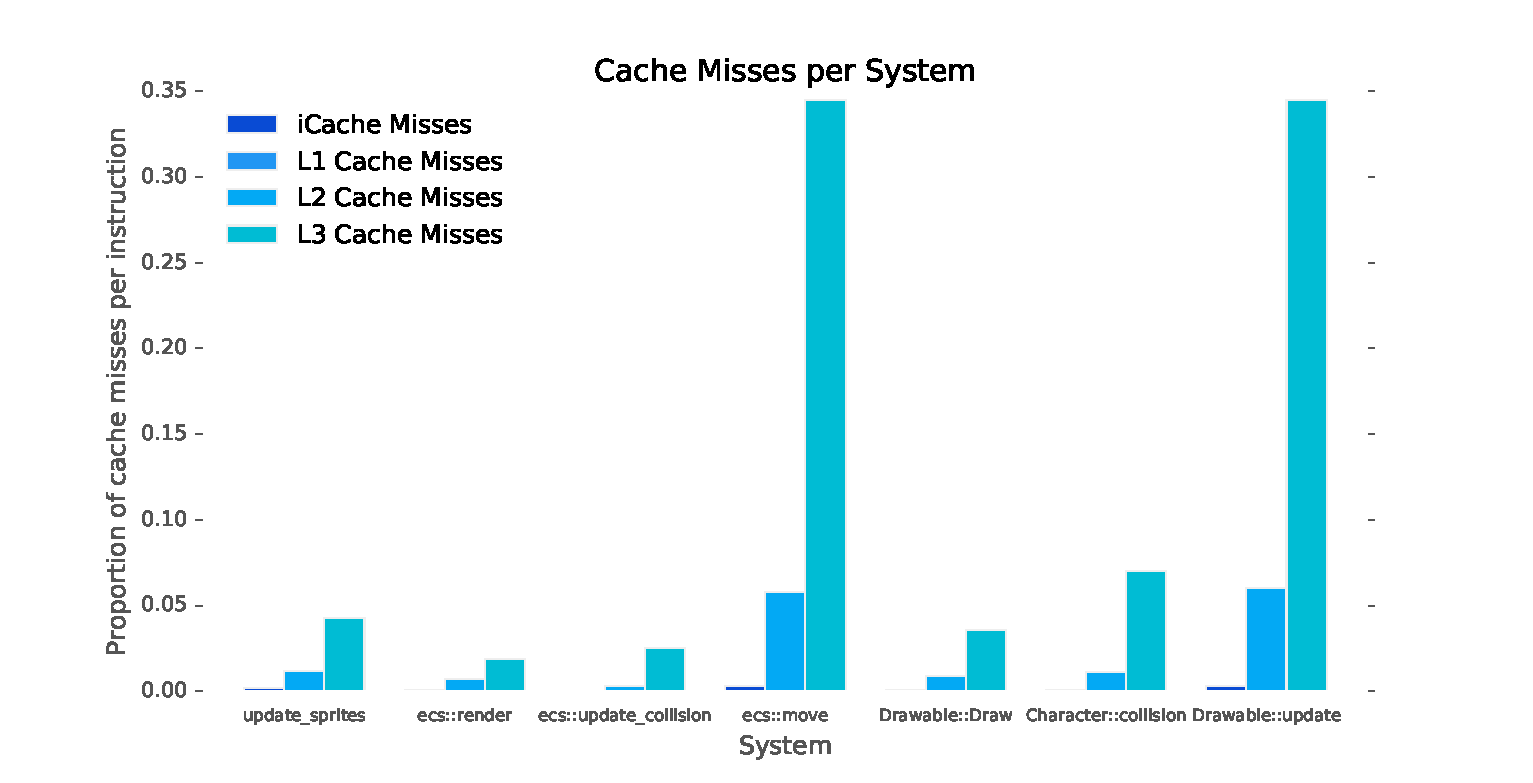
\includegraphics[width=\textwidth]{profiling/individual.eps}
	\caption{Cache misses per cache per instruction for each system}
	\label{fig:function_misses}
\end{figure}
% section appendix_b_results (end)

\end{document}